\documentclass[11pt]{article}

\usepackage[margin=1in,letterpaper]{geometry}
\usepackage{amsmath}%,bm}
\usepackage{mathtools}
%\usepackage{siunitx}
\usepackage{enumitem}
%\usepackage{graphicx}
\usepackage{tikz}
\usepackage{mathpazo}
%\usepackage{xcolor,colortbl}
%\usepackage{hyperref}
\usepackage{cancel}

\newcommand\vertarrowbox[2]{%
    \begin{array}[t]{@{}c@{}} #1 \\
    \rotatebox{90}{$\xrightarrow{\hphantom{abcdefgh}}$} \\[-1ex]
    \mathclap{\scriptstyle\text{#2}}%
    \end{array}}

\setlength{\parindent}{0pt}
\setlength{\parskip}{8pt}

%\usetikzlibrary{decorations.pathmorphing,patterns}

%\sisetup{
%  detect-all,
%  number-math-rm=\mathnormal,
%  per-mode=symbol
%}

\title{One-Dimensional Motion Graphs for Constant Acceleration}
\author{Timothy M.\ Leung, Ph.D.\\Olympiads School}
\date{\today}

%\newcommand{\pic}[2]{
%  \includegraphics[width=#1\textwidth]{#2}
%}
%\newcommand{\mb}[1]{
%  \ensuremath\mathbf{#1}
%}

\begin{document}
\maketitle

\textbf{THIS IS THE FIRST DRAFT OF A LONGER HANDOUT. AT THE MOMENT, THERE ARE
  STILL SOME INFORMATION MISSING.}

In analyzing one-dimensional motion, particularly in experiments, we often use
\textbf{motion graphs} to graphically express how motion quantities (position,
velocity, acceleration) evolves in time. The basic motion graphs most familiar
to physics students are:
\begin{itemize}[noitemsep,topsep=0pt,leftmargin=15pt]
\item position vs.\ time (or displacement vs.\ time)
\item velocity vs.\ time
\item acceleration vs.\ time
\end{itemize}
Since velocity is the time derivative of position ($v=\dot{x}$), and
acceleration is the time derivative of velocity ($a=\dot{v}=\ddot{x}$), the
relationship between the graphs are straightforward: the velocity graph is the
slope of the position graph, and the acceleration graph is the slope of the
velocity graph. We can also use the area under the acceleration graph to find
the change in velocity ($\int a(t)dt=\Delta v$) and the area under the velocity
graph to find displacement ($\int v(t)dt=\Delta x$).

\section{Graphs for Uniform Motion \& Uniform Acceleration}
For uniform motion (constant velocity), the basic motion graphs are shown in
Figure~\ref{uniform-motion}. All the graphs are linear. Computing the slopes
(derivatives) and areas (integrals) are straightforward exercises.
\begin{figure}[!ht]
  \centering
  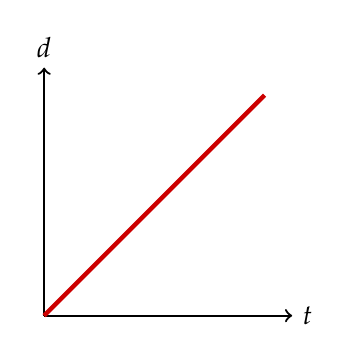
\begin{tikzpicture}[scale=.7]
    \draw[->,thick] (0,0)--(4.5,0) node[pos=1,right]{$t$};
    \draw[->,thick] (0,0)--(0,4.5) node[pos=1,above]{$d$};
    \draw[red!80!black,ultra thick](0,0)--(4,4);
  \end{tikzpicture}
  \hspace{.15in}
  \begin{tikzpicture}[scale=.7]
    \draw[->,thick] (0,0)--(4.5,0) node[pos=1,right]{$t$};
    \draw[->,thick] (0,0)--(0,4.5) node[pos=1,above]{$v$};
    \draw[red!80!black,ultra thick](0,2)--(4,2);
  \end{tikzpicture}
  \hspace{.15in}
  \begin{tikzpicture}[scale=.7]
    \draw[->,thick] (0,0)--(4.5,0) node[pos=1,right]{$t$};
    \draw[->,thick] (0,0)--(0,4.5) node[pos=1,above]{$a$};
    \draw[red!80!black,ultra thick](0,0)--(4,0);
  \end{tikzpicture}
  \caption{Position, velocity and acceleration are all linear functions of time
    for uniform motion.}
  \label{uniform-motion}
\end{figure}

For uniform acceleration, the position graph is a parabola, while velocity and
acceleration graphs are linear, as shown in Figure~\ref{uniform-acceleration}.
Computing the area under the velocity and acceleration graphs are still
straightforward, as is finding the slope of the velocity graph, however,
finding the acceleration using only the position graph is much more difficult.
\begin{figure}[!ht]
  \centering
  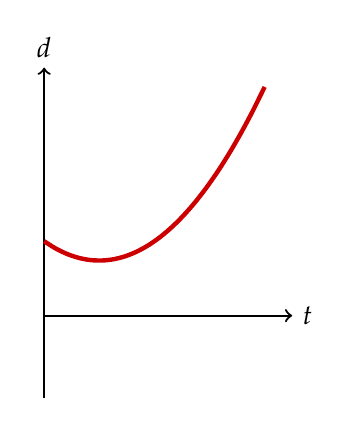
\begin{tikzpicture}[scale=.7]
    \draw[->,thick] (0,0)--(4.5,0) node[pos=1,right]{$t$};
    \draw[->,thick] (0,-1.5)--(0,4.5) node[pos=1,above]{$d$};
    \draw[smooth,samples=20,domain=0:4,red!80!black,ultra thick]
    plot({\x},{0.35*(\x-1)*(\x-1)+1});
  \end{tikzpicture}
  \hspace{.15in}
  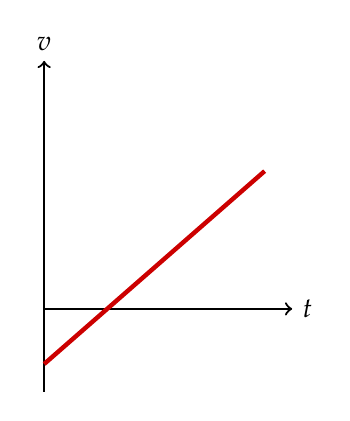
\begin{tikzpicture}[scale=.7]
    \draw[->,thick] (0,0)--(4.5,0) node[pos=1,right]{$t$};
    \draw[->,thick] (0,-1.5)--(0,4.5) node[pos=1,above]{$v$};
    \draw[red!80!black,ultra thick](0,-1)--(4,2.5);
  \end{tikzpicture}
  \hspace{.15in}
  \begin{tikzpicture}[scale=.7]
    \draw[->,thick] (0,0)--(4.5,0) node[pos=1,right]{$t$};
    \draw[->,thick] (0,-1.5)--(0,4.5) node[pos=1,above]{$a$};
    \draw[red!80!black,ultra thick](0,1)--(4,1);
  \end{tikzpicture}
  \caption{Displacement, velocity and acceleration as functions of time for
    uniformly accelerated motion.}
  \label{uniform-acceleration}
\end{figure}


\section{Position vs. Time Squared}
In many cases, the position graph in Figure~\ref{uniform-acceleration} is
obtained experimentally by plotting values of $x$ and $t$, and then making
curve fit of the data, by making an educated guess that acceleration is
uniform\footnote{This would have to be done through a thorough analysis of all
  the forces acting on an object.}, and therefore the graph is a parabola.
However, one of the weaknesses of this graph is the difficulty in determining
the acceleration of the object by examining the graph itself. It is possible to
take the second time derivative of the fitted curve to calculate the
acceleration, which must be known algebraically in order to be plotted.
Inevitably, some accuracy will be lost.

One way to get around the problem is that, \emph{if initial velocity is zero},
i.e.\ $v_0=0$, then instead of plotting position $x$ directly against time $t$,
we re-interpret the the kinematic equation as a linear function in the form
of $y=mx+b$:
\begin{equation}
  \vertarrowbox{x}{y}=\vertarrowbox{\left(\frac12 a\right)}{m}
  \vertarrowbox{t^2}{x}+
  \cancel{v_0t}+
  \vertarrowbox{x_0}{b}
\end{equation}
and plot $x$ against the \emph{square} of time, $t^2$. If acceleration is
indeed uniform, then the graph would be linear. That constant acceleration is
twice slope, i.e.:
\begin{equation*}
  m=\frac12 a\quad\rightarrow\quad a=2m
\end{equation*}
The $x$-intercept of both graphs are still the initial position $x_0$. One
example is shown in Figure~\ref{switch1}. The $x$ vs.\ $t$ and the $x$ vs.\
$t^2$ graphs both describe the same motion.
\begin{figure}[!ht]
  \centering
  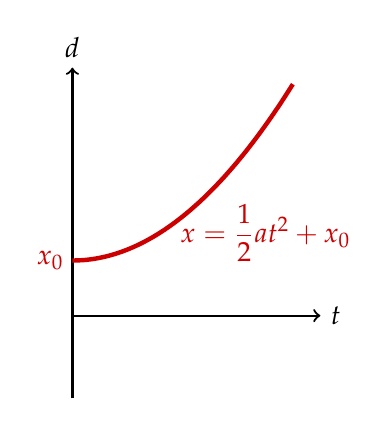
\begin{tikzpicture}[scale=.7]
    \draw[->,thick] (0,0)--(4.5,0) node[pos=1,right]{$t$};
    \draw[->,thick] (0,-1.5)--(0,4.5) node[pos=1,above]{$d$};
    \draw[smooth,samples=20,domain=0:4,red!80!black,ultra thick]
    plot({\x},{.2*(\x)*(\x)+1});
    \node[red!80!black] at (3.5,1.5) {$\displaystyle x=\frac12at^2+x_0$};
    \node[red!80!black] at (-.4,1) {$x_0$};
  \end{tikzpicture}
  \hspace{.15in}
  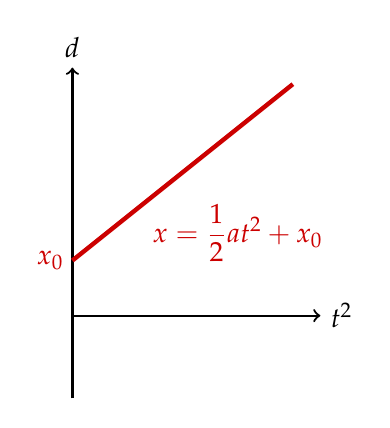
\begin{tikzpicture}[scale=.7]
    \draw[->,thick] (0,0)--(4.5,0) node[pos=1,right]{$t^2$};
    \draw[->,thick] (0,-1.5)--(0,4.5) node[pos=1,above]{$d$};
    \draw[red!80!black,ultra thick](0,1)--(4,4.2);
    \node[red!80!black] at (3,1.5) {$\displaystyle x=\frac12at^2+x_0$};
    \node[red!80!black] at (-.4,1) {$x_0$};
  \end{tikzpicture}
  \caption{Position plotted against time $t$ and time squared $t^2$ for
    uniformly accelerated motion.}
  \label{switch1}
\end{figure} 


\section{Velocity Squared vs.\ Displacement}
Likewise, some experimental equation is able to capture velocity information
as an object moves in \emph{space}. In other words, velocity and position
information is available experimentally but not time, then instead of plotting
velocity vs.\ time, position vs.\ time, we can plot velocity as a function of
\emph{position}. Again, even if acceleration is uniform, finding $a$ from this
graph is not straightforward. However, another option is to, like in the
previous section, re-interpret the kinematic equation as a linear function:
\begin{equation}
  \vertarrowbox{v^2}{$y$}=
  \vertarrowbox{v_0^2}{b}+\vertarrowbox{(2a)}{m}
  \vertarrowbox{(x-x_0)}{x}
\end{equation}
and plot the \emph{square} of velocity (i.e.\ $v^2$) as a function of
displacement ($x-x_0$). If acceleration is uniform (constant $a$), the graph
would be linear. The acceleration is half the slope $m$ of the graph:
$\displaystyle a=\frac{m}{2}$ and the $y$-intercept is the square of the
initial velocity (i.e.\ $v_0^2$).
\end{document}
